%-----------------------------------------------------------------------------
%
%               Template for sigplanconf LaTeX Class
%
% Name:         sigplanconf-template.tex
%
% Purpose:      A template for sigplanconf.cls, which is a LaTeX 2e class
%               file for SIGPLAN conference proceedings.
%
% Guide:        Refer to "Author's Guide to the ACM SIGPLAN Class,"
%               sigplanconf-guide.pdf
%
% Author:       Paul C. Anagnostopoulos
%               Windfall Software
%               978 371-2316
%               paul@windfall.com
%
% Created:      15 February 2005
%
%-----------------------------------------------------------------------------


\documentclass[preprint]{sigplanconf}

% The following \documentclass options may be useful:

% preprint      Remove this option only once the paper is in final form.
% 10pt          To set in 10-point type instead of 9-point.
% 11pt          To set in 11-point type instead of 9-point.
% authoryear    To obtain author/year citation style instead of numeric.

\let\program\undefined % \program from acmtras2e conflicts with our program

\usepackage{amsmath}
\usepackage{program}
\usepackage{graphicx}

% hyphen-able fixed-width font
\newcommand{\ttt}[1]{{\texttt{\hyphenchar\font=`\-\relax #1}}}%`
\newcommand{\fixme}[1]{{\color{red} #1}}

\begin{document}

\special{papersize=8.5in,11in}
\setlength{\pdfpageheight}{\paperheight}
\setlength{\pdfpagewidth}{\paperwidth}

\conferenceinfo{Workshop on Programming Models for SIMD/Vector Processing - WPMVP'15}{February 7--8, 2015, San Francisco, CA, USA} 
\copyrightyear{2015} 
\copyrightdata{978-1-nnnn-nnnn-n/15/2} 
\doi{nnnnnnn.nnnnnnn}

% Uncomment one of the following two, if you are not going for the 
% traditional copyright transfer agreement.

%\exclusivelicense                % ACM gets exclusive license to publish, 
                                  % you retain copyright

%\permissiontopublish             % ACM gets nonexclusive license to publish
                                  % (paid open-access papers, 
                                  % short abstracts)

\titlebanner{DRAFT}        % These are ignored unless
\preprintfooter{SIMD in JavaScript via C++ and Emscripten}   % 'preprint' option specified.

\title{SIMD in JavaScript via C++ and Emscripten}
% \subtitle{Subtitle Text, if any}

\authorinfo{Peter Jensen}
           {Intel Corporation}
           {peter.jensen@intel.com}
\authorinfo{John McCutchan}
           {Google Inc.}
           {johnmccutchan@google.com}
\authorinfo{Ivan Jibaja}
           {Intel Corporation}
           {ivan.jibaja@intel.com}
\authorinfo{Dan Gohman}
           {Mozilla}
           {sunfish@mozilla.com}
\authorinfo{Ningxin Hu}
           {Intel Corporation}
           {ningxin.hu@intel.com}

\maketitle

\begin{abstract}
This is the text of the abstract.
\end{abstract}

%\category{CR-number}{subcategory}{third-level}

% general terms are not compulsory anymore, 
% you may leave them out
%\terms
%term1, term2

%\keywords
%keyword1, keyword2

\section{Introduction}

We'll explore the use of Mozilla's Emscripten to compile C++ programs, that
has use of SIMD intrinsics or gcc style vector code, into JavaScript.  This was
recently made possible by the SIMD.JS primitives introduced in JavaScript 
engine prototypes for Chromium and Firefox as well as extensions to the 
Emscripten compiler.  Emscripten will correctly translate a subset of available
C++ SIMD x86 intrinsics into corresponding operations defined in SIMD.JS. The
JavaScript benchmarks associated with the SIMD.JS primitives were converted to 
C++ by hand, and then automatically converted back into JavaScript using the 
Emscripten compiler.

\section{SIMD.JS}

SIMD is short for Single Instruction, Multiple Data.  It refers to CPU 
instruction level data parallelism.  Most modern CPUs have a significant 
portion of their available instructions dedicated to operating on data in
parallel.  Typically, those instructions will perform the same operation on 
elements in short vectors, e.g. vectors of length 4, 8, or 16.  Use of these 
instructions leads to increased performance, because more data processing is 
achieved with fewer instructions executed, and fewer instructions also means
power savings, which is of outmost importance on mobile battery powered
devices.  Figure~\ref{fig:simd} shows how four scalar additions are 
combined into a single operation.

\begin{figure}
\begin{center}
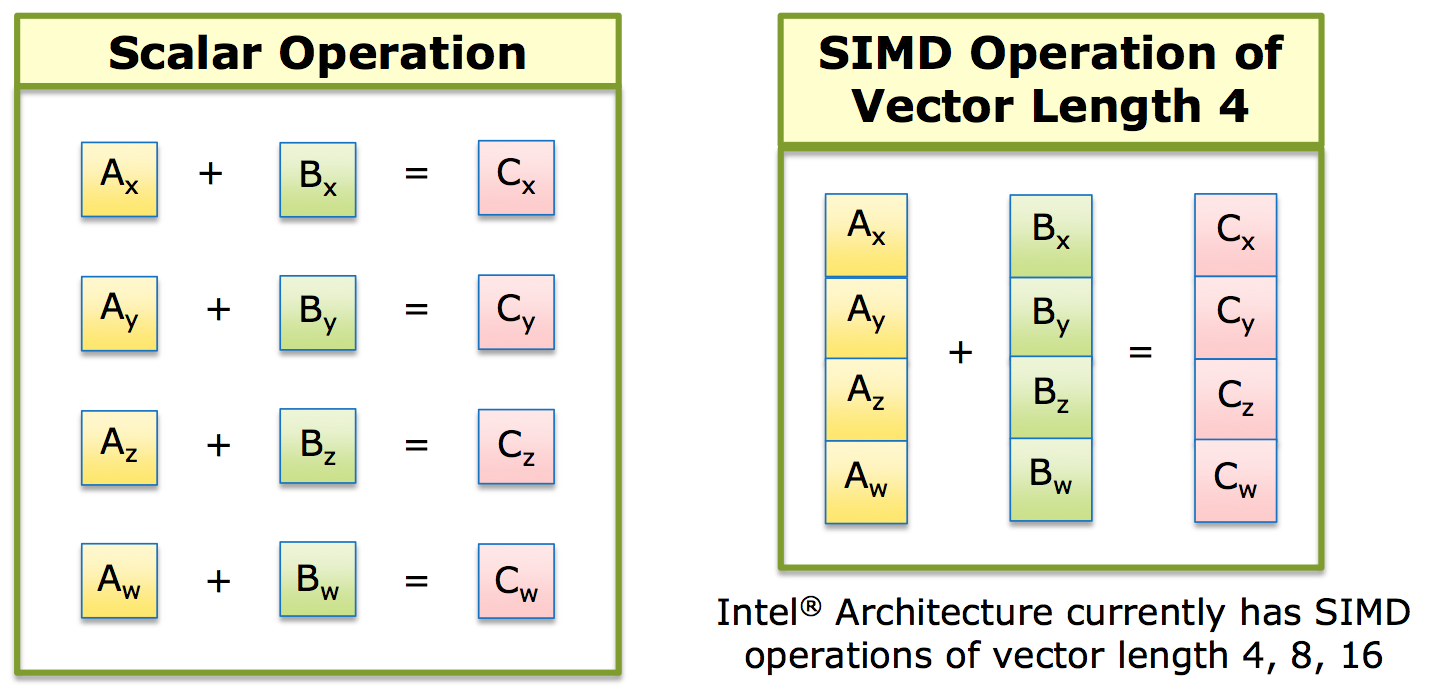
\includegraphics[width=0.45\textwidth]{figures/simd-04.png}
\end{center}
\caption{Replacing four scalar additions with one SIMD addition}
\label{fig:simd}
\end{figure}

JavaScript is quickly emerging as one of the most popular languages among 
software developers.  It was originally used for simple web page scripting for 
creating interactive web pages. Around 2008, very efficient and high 
performance JavaScript engines emerged, e.g. Firefox's TraceMonkey and 
Chrome's V8 engines. Since then, JavaScript has become a viable language for 
things beyond just basic web page interactivity, as witnessed by it's use in 
large web based applications, such as office applications; e-mail, document 
processing, etc. Also, large games, which were previously standalone, natively
compiled programs, have been ported to JavaScript to run within the browser 
environment.  More recently, JavaScript has been adopted as a server side 
scripting language (node.js), and lately, JavaScript has found it's way to the
mobil platform as a language that offers better portability between the 
different mobile platforms without sacrificing performance and features.  For 
example, access to platform sensors (location, accelerometers, etc) are 
accessible from JavaScript via W3C APIs.

Even with the past 7 years of JavaScript performance advances, the desire for 
better performing JavaScript engines has not lessened, quite the contrary. It's
a spiral that keeps on going; better performance leads to more uses, more uses 
require better performance.  Specifically, software that use data parallelism 
to achieve adequate performance have, so far, been restricted to natively 
compiled languages, such as C++, because such languages offer ways of utilizing 
the SIMD instructions available in modern CPUs.  JavaScript has only one number
type, Number, which is an IEEE-754 floating point number, and JavaScript offers 
no abstraction primitives for writing algorithms utilizing data paralellism, so 
it's imperative that this shortcoming is dealt with, such that the next leap
in JavaScript performance is made possible.  This is what the SIMD.JS proposal
addresses.

SIMD.JS is an emerging standard developed collaboratively by Intel,
Mozilla, Google, and Microsoft.  It provides low level data types and 
operations that map well onto the available SIMD instructions of the underlying 
hardware.  Currently, the defined data types and operations are a 
representative and useful overlap between SIMD types and operations available 
in most modern CPUs.

The SIMD.JS proposal is structured as an object hierarchy, with SIMD being the
top level global object.  The immediate properties of the SIMD object reflect
the data types; \ttt{int32x4}, \ttt{float32x4}, and \ttt{float64x2}.  The 
operations are methods declared as properties on the data type properties as 
outlined in  Figure~\ref{fig:hierarchy}, which shows a portion of the object 
hierarchy.

\begin{figure}
\begin{center}
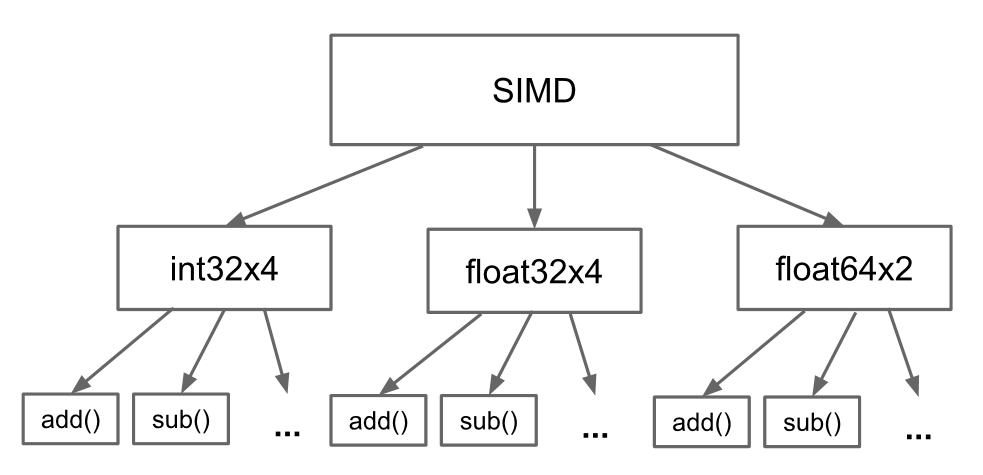
\includegraphics[width=0.45\textwidth]{figures/hierarchy.png}
\end{center}
\caption{SIMD.JS object hierarchy}
\label{fig:hierarchy}
\end{figure}

We've modelled the semantics of the SIMD types and operations as a polyfill 
<REF>.  This allows programmers to experiment without using a JavaScript
engine that natively supports SIMD.JS.  The polyfill also serves as documentation
for the semantics and interfaces.  It will also reflect the current state of
the proposal.  The proposal is under active development and changes are likely to 
happen as the proposal is being refined and moves forward through the approval
process.

As an example use case, Figure~\ref{fig:simd-average} shows the SIMD JavaScript
code for computing the average of an array of floating point numbers.  The numbers
are held in a Float32Array typed array; \ttt{data}.  The benefit of using SIMD 
operations, for computing the average, is that four numbers can be added in one
operation, thereby reducing the number of iterations by a factor of 4, and 
achieving an equivalent speedup.

\begin{figure}
\begin{small}
\begin{program}[style=tt, number=true]
fu\tab{}nction average(data) \{
  var sum = SIMD.float32x4.splat(0.0);
  fo\tab{}r (var i = 0, l = data.length; i < l; i = i+4) \{
    su\tab{}m = SIMD.float32x4.add(
      sum, SIMD.float32x4.load(data, i));\untab{}\untab{}
  \}
  var total = sum.x + sum.y + sum.z + sum.w;
  return total/data.length;\untab{}
\}
\end{program}
\end{small}
\caption{Finding the average of an array of numbers in JavaScript using SIMD}
\label{fig:simd-average}
\end{figure}

The optimizing Just-In-Time (JIT) compiler in our Chrome/V8 SIMD enabled
prototype is able to produce the code in Figure~\ref{simd-average-code} for
the body of the loop.  The code shows how the compiler is able utilize a
128-bit SIMD register (xmm) to hold the value of \ttt{sum} and to use the
\ttt{addps} instruction for adding 4 single precision numbers in one
instruction.  For more details on how the JIT compilers operate see <REF>.

\begin{figure}
\begin{small}
\begin{program}[style=tt, number=true]
Assembly dump
\end{program}
\end{small}
\caption{JIT compiler generated code for the \ttt{average} function}
\label{fig:simd-average-code}
\end{figure}

\subsection{The Future of SIMD.JS}

The proposal has been presented to TC39, the JavaScript language standard
commitee, and was unanimously approved for stage 1 in 2014.  Stage 1 is the
proposal stage.  It indicates that the need has been justified, and an 
outline for a solution has been accepted.  It does not mean that this is the final
proposal.

The focus, so far, has been on identifying types and operations that can be
effectively implemented on all relevant CPU architectures.  We realize that CPUs
have destinct features that are useful and it will make sense to expose such 
features to the JavaScript programmer.  This will most likely be done via
architecture specific extensions to the SIMD object, e.g. SIMD.x86.*

SIMD.JS is currently being refined and prepared for the next stages of approval,
and we expect this to be part of the EcmaScript 7 standard (ES7).
EcmaScript 5 is the current JavaScript standard.  EcmaScript 6 is slated for a
mid-2015 release. ES6 is a major overhaul of the JavaScript language and a 
substantial set of new features were added, as reflected by the size of the 
language specification document.  The ES5 specification document is roughly 300 
pages, whereas the ES6 specification is roughly double that. Most browsers 
have already implemented most of the ES6 features.

\section{Emscripten}

\section{Compiling x86 C++ SIMD intrinsics}

\section{Benchmarks}

\section{Results}

\section{Summary}

\appendix
\section{Appendix Title}

This is the text of the appendix, if you need one.

\acks

Acknowledgments, if needed.

% We recommend abbrvnat bibliography style.

\bibliographystyle{abbrvnat}

% The bibliography should be embedded for final submission.

\begin{thebibliography}{}
\softraggedright

\bibitem[Smith et~al.(2009)Smith, Jones]{smith02}
P. Q. Smith, and X. Y. Jones. ...reference text...

\end{thebibliography}


\end{document}

%                       Revision History
%                       -------- -------
%  Date         Person  Ver.    Change
%  ----         ------  ----    ------

%  2013.06.29   TU      0.1--4  comments on permission/copyright notices

